% select subfiles base file
\documentclass[TGAI_Laborbericht.tex]{subfiles}
\begin{document}

%\phantomsection
\chapter*{Anhang}
\label{chap:APPENDIX}
\addcontentsline{toc}{chapter}{Anhang}
%\setcounter{chapter}{0}
\addtocounter{chapter}{1}
\setcounter{section}{0}

\section{Quellcode}
\label{chap:APPENDIX_SOURCECODE}

\subsection{Quellcode Versuch 1}
\label{chap:APPENDIX_SOURCECODE_V1}
\lstinputlisting[language=python]{media/v5.py}


\section{Messergebnisse}
\label{chap:APPENDIX_MEASUREMENT_SOURCE}
\begin{figure}[H]
	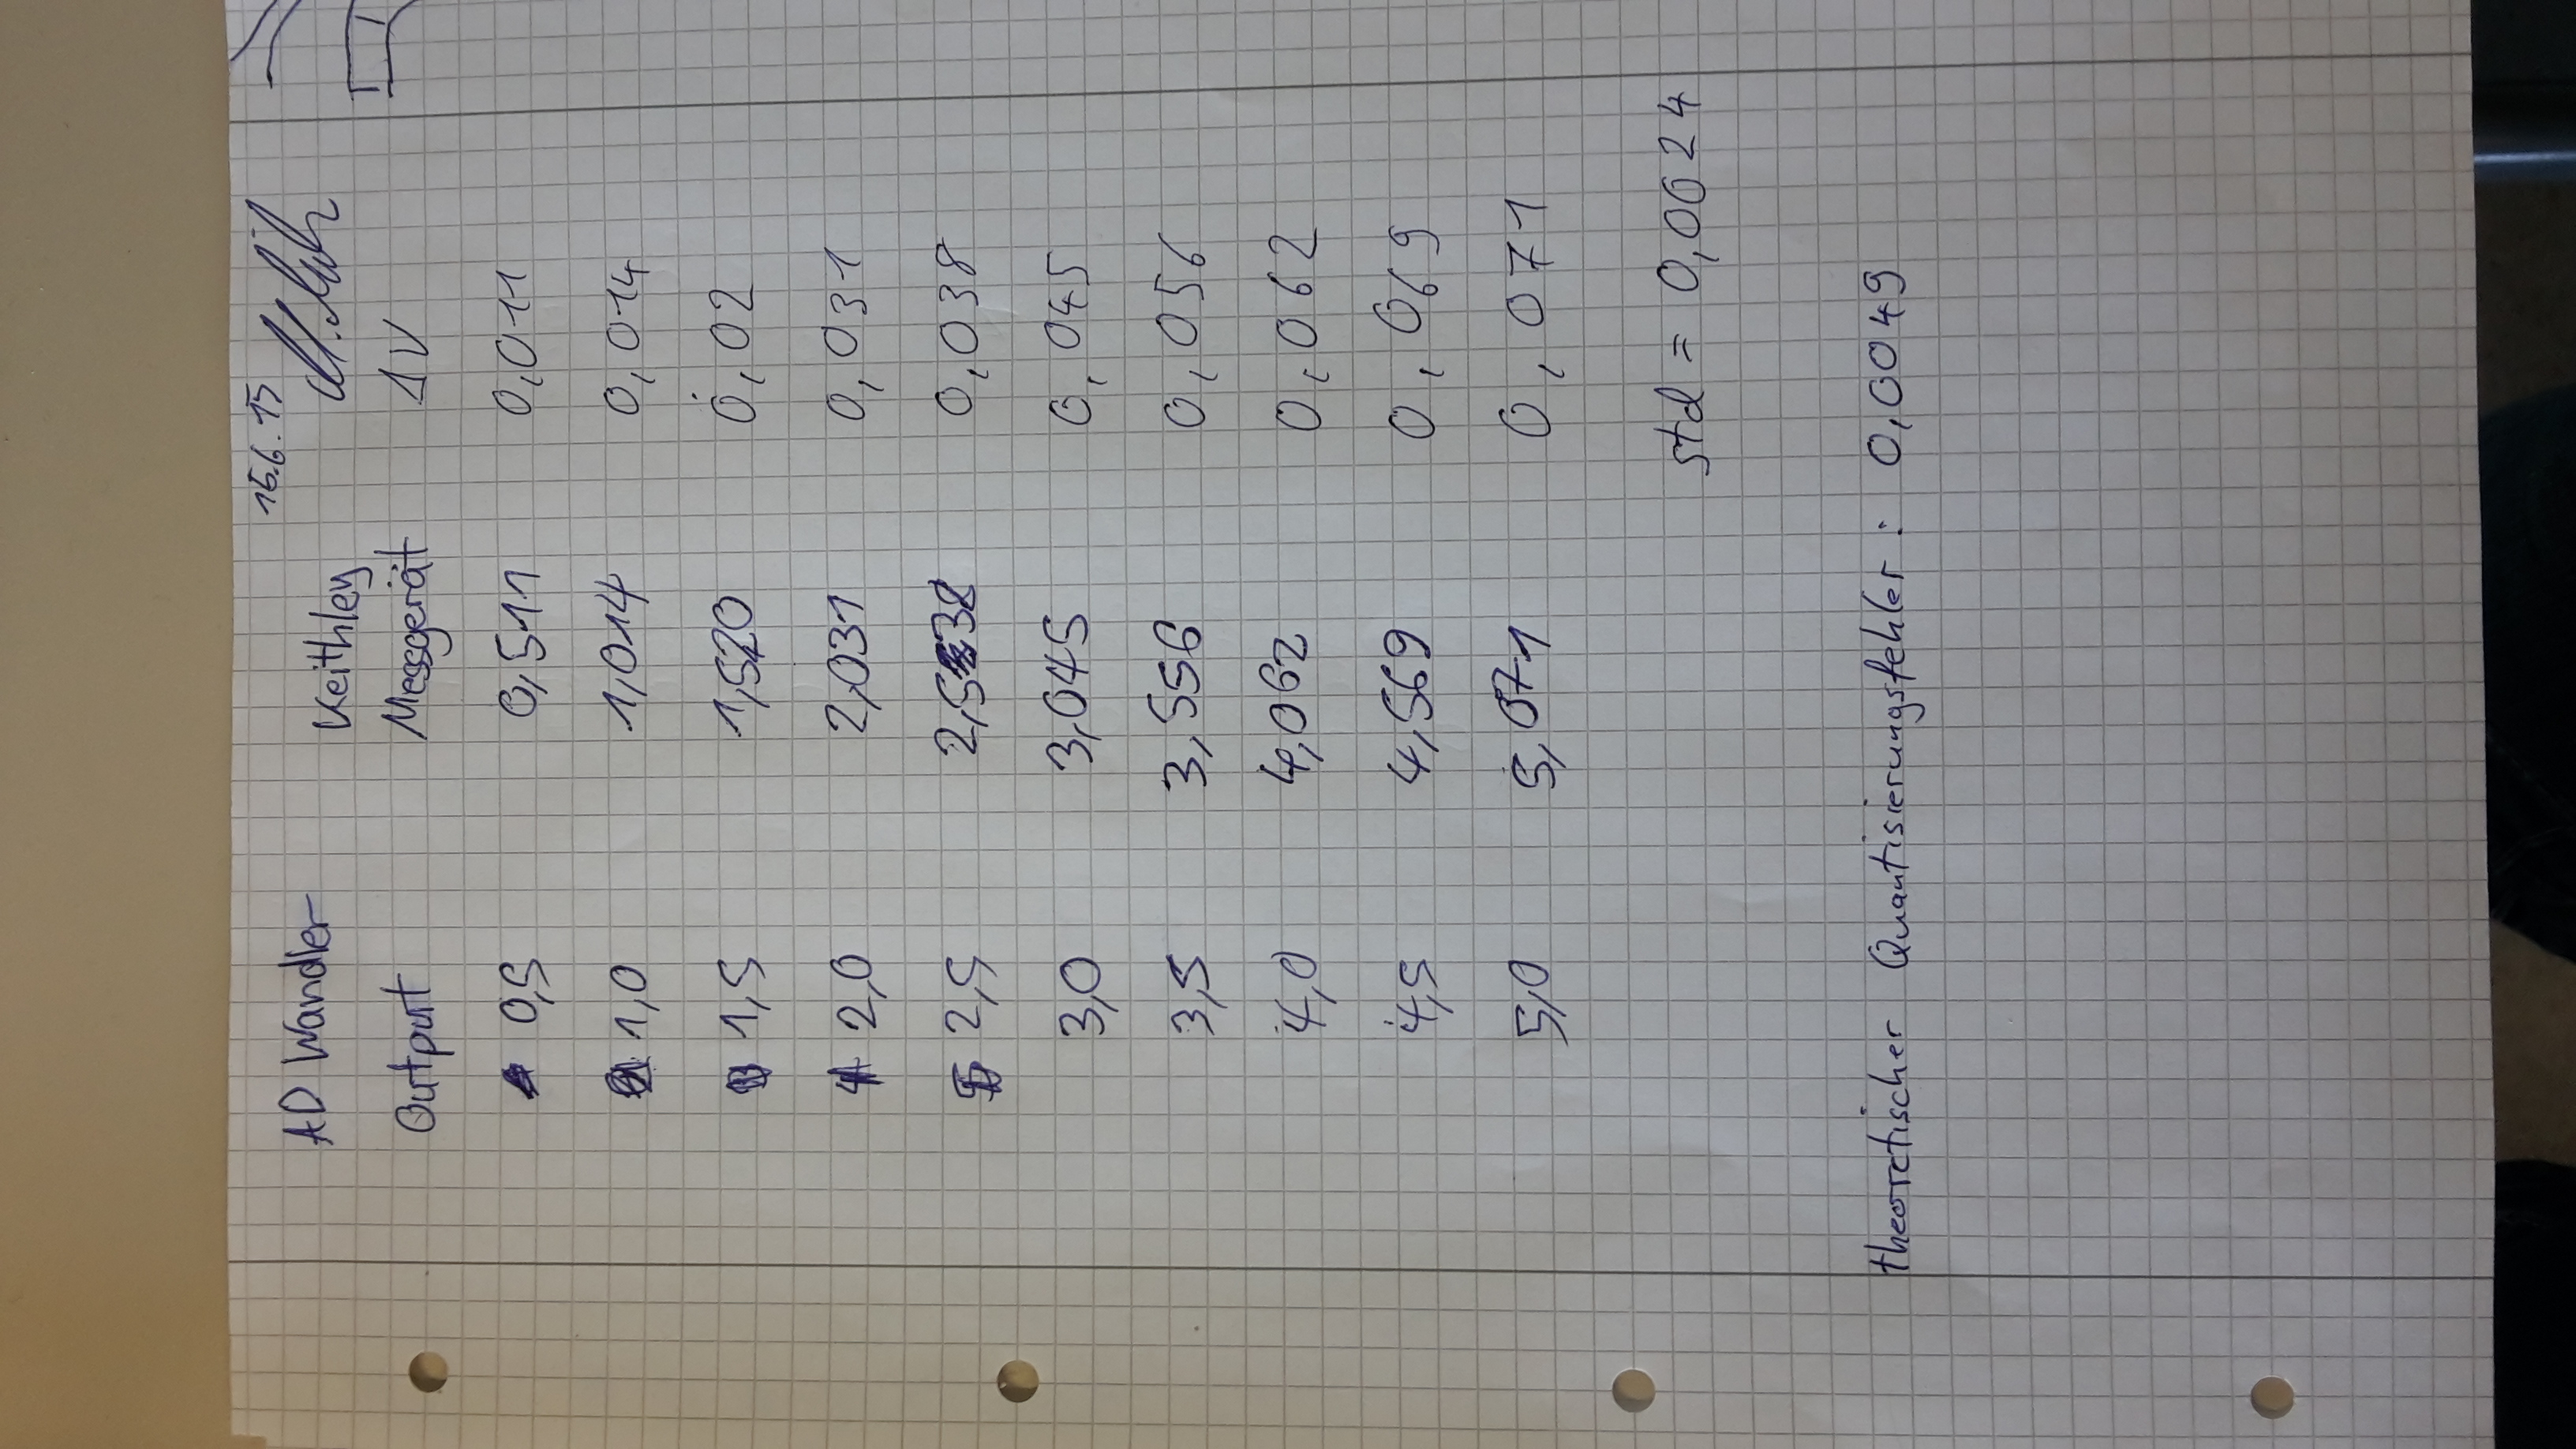
\includegraphics[width=1.5\textwidth, angle = -90]{media/Messprotokoll1.jpg}
	\label{Output}
	\caption{Messprotokoll D/A Output}
\end{figure}
\begin{figure}[H]
	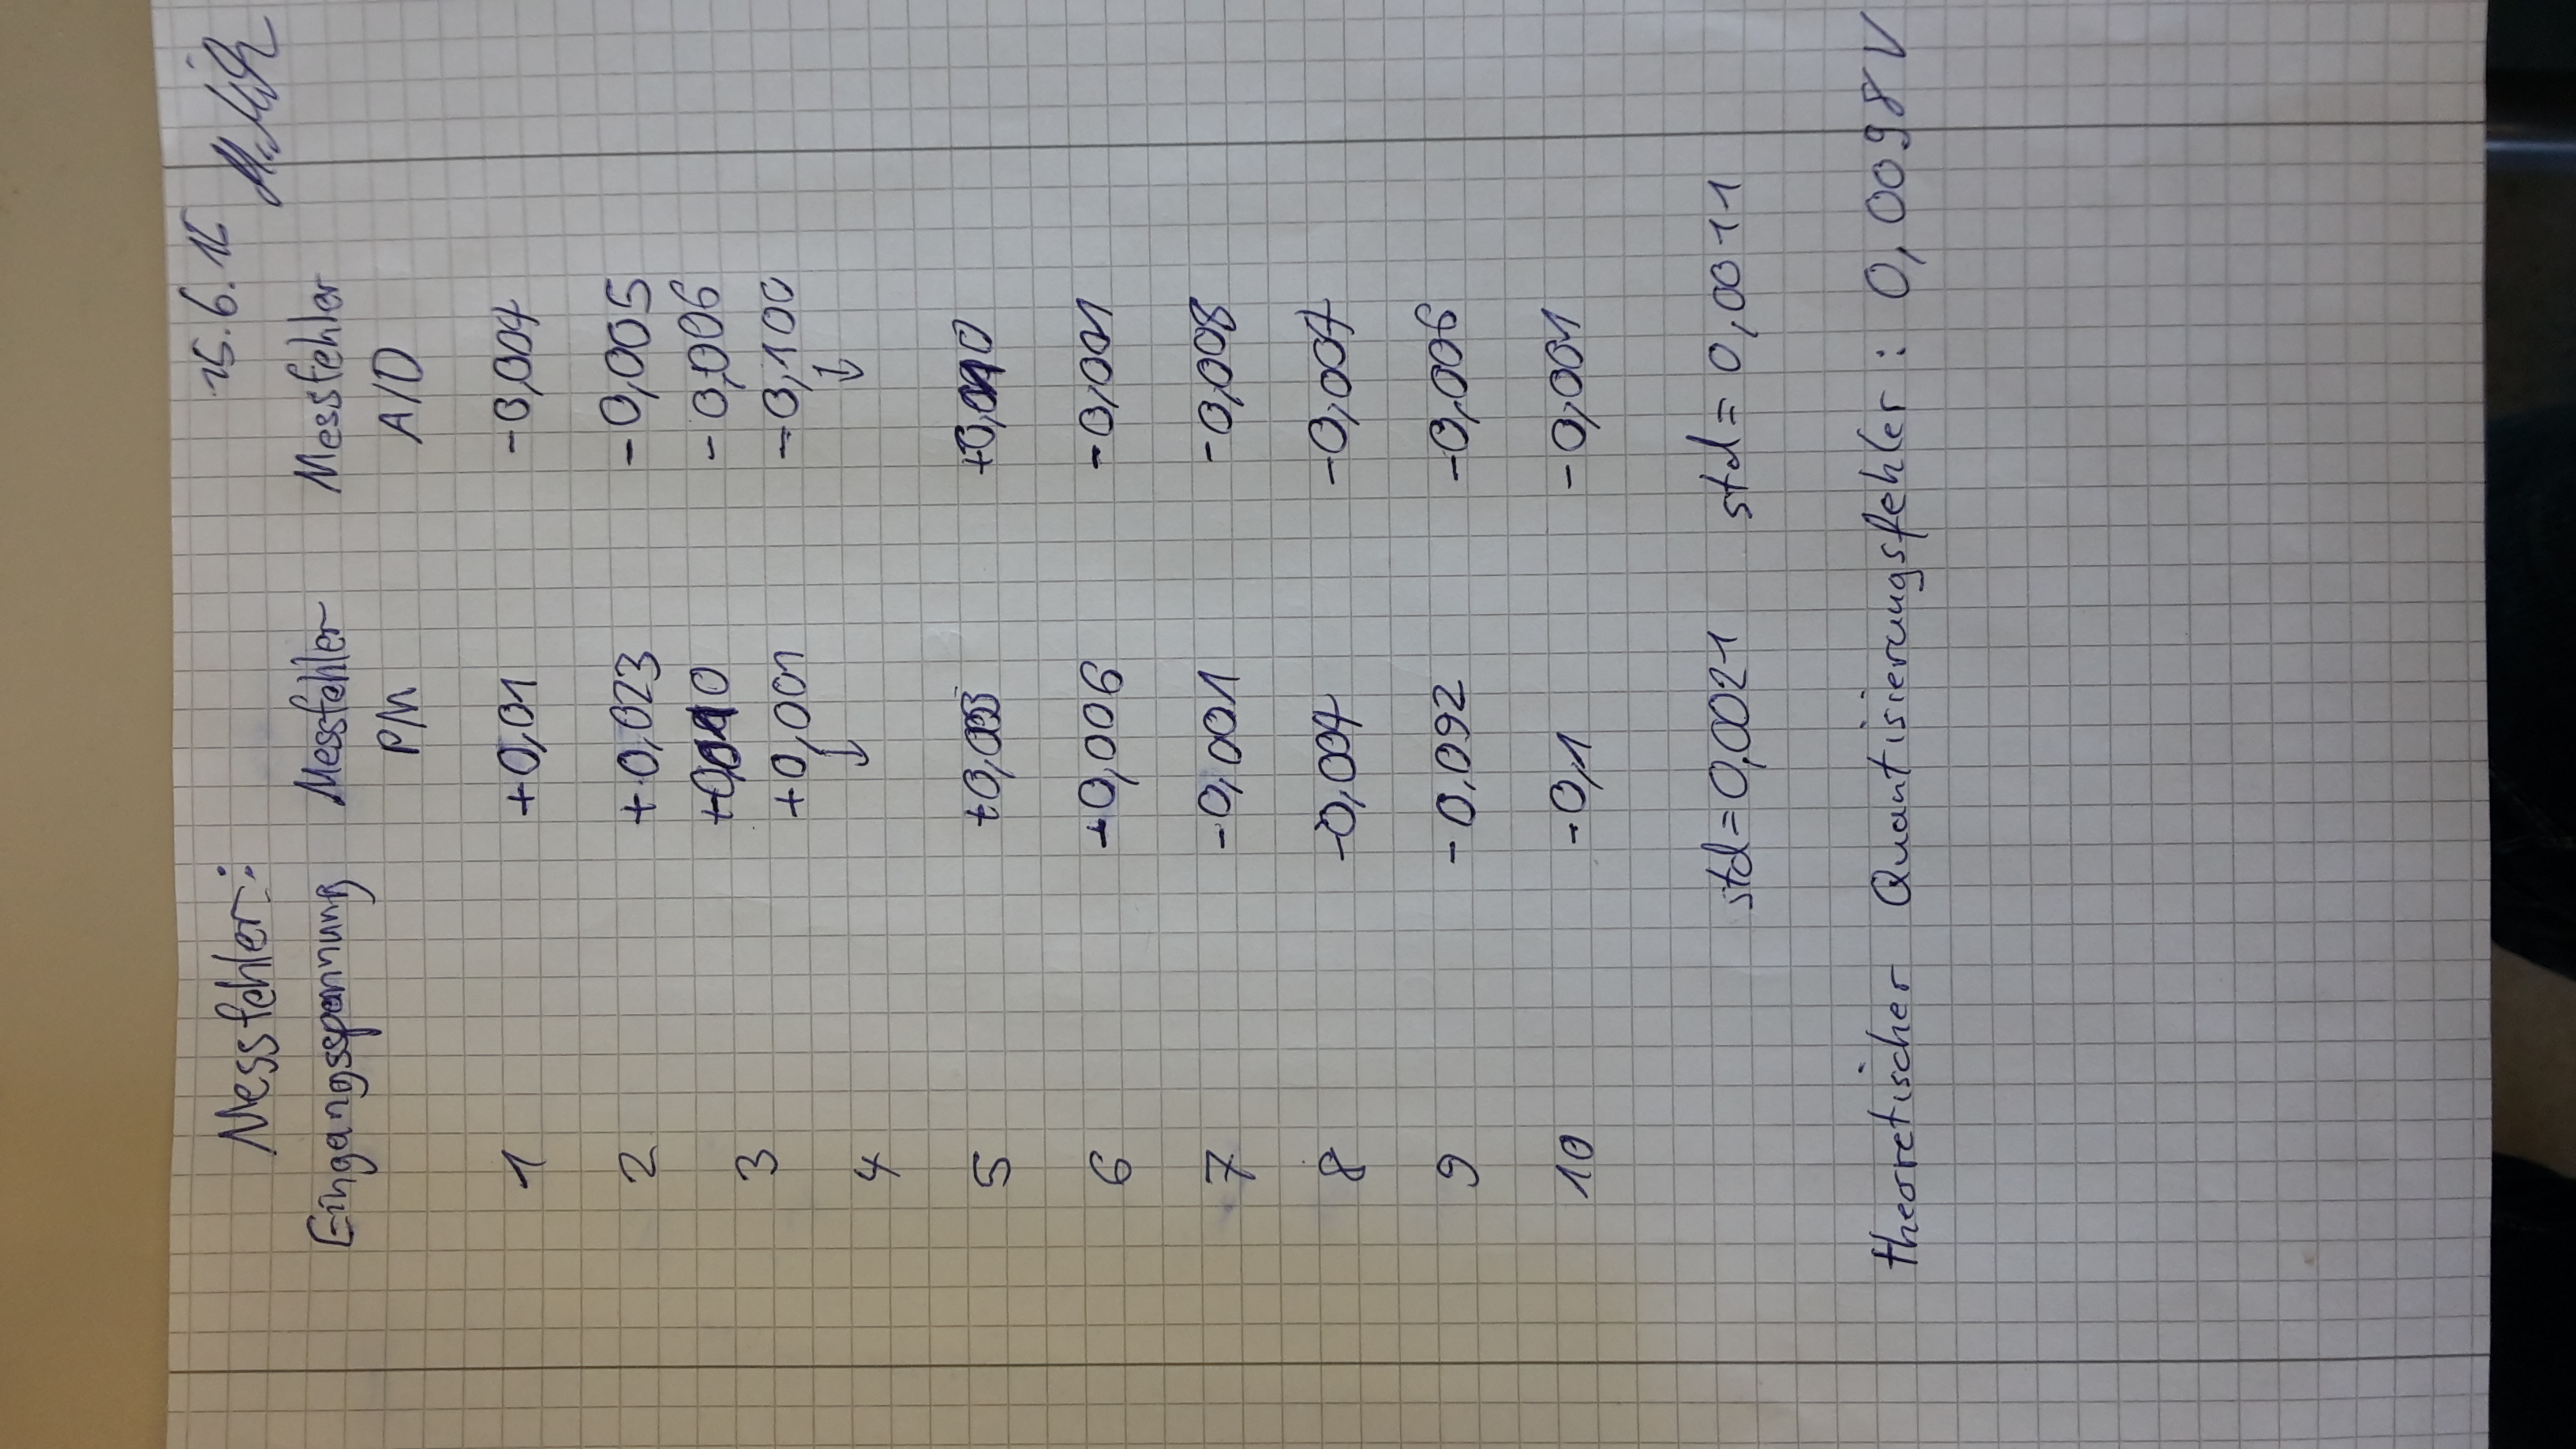
\includegraphics[width=1.5\textwidth, angle = -90]{media/Messprotokoll2.jpg}
	\label{Messfehler}
	\caption{Messfehler}
\end{figure}
\begin{figure}[H]
	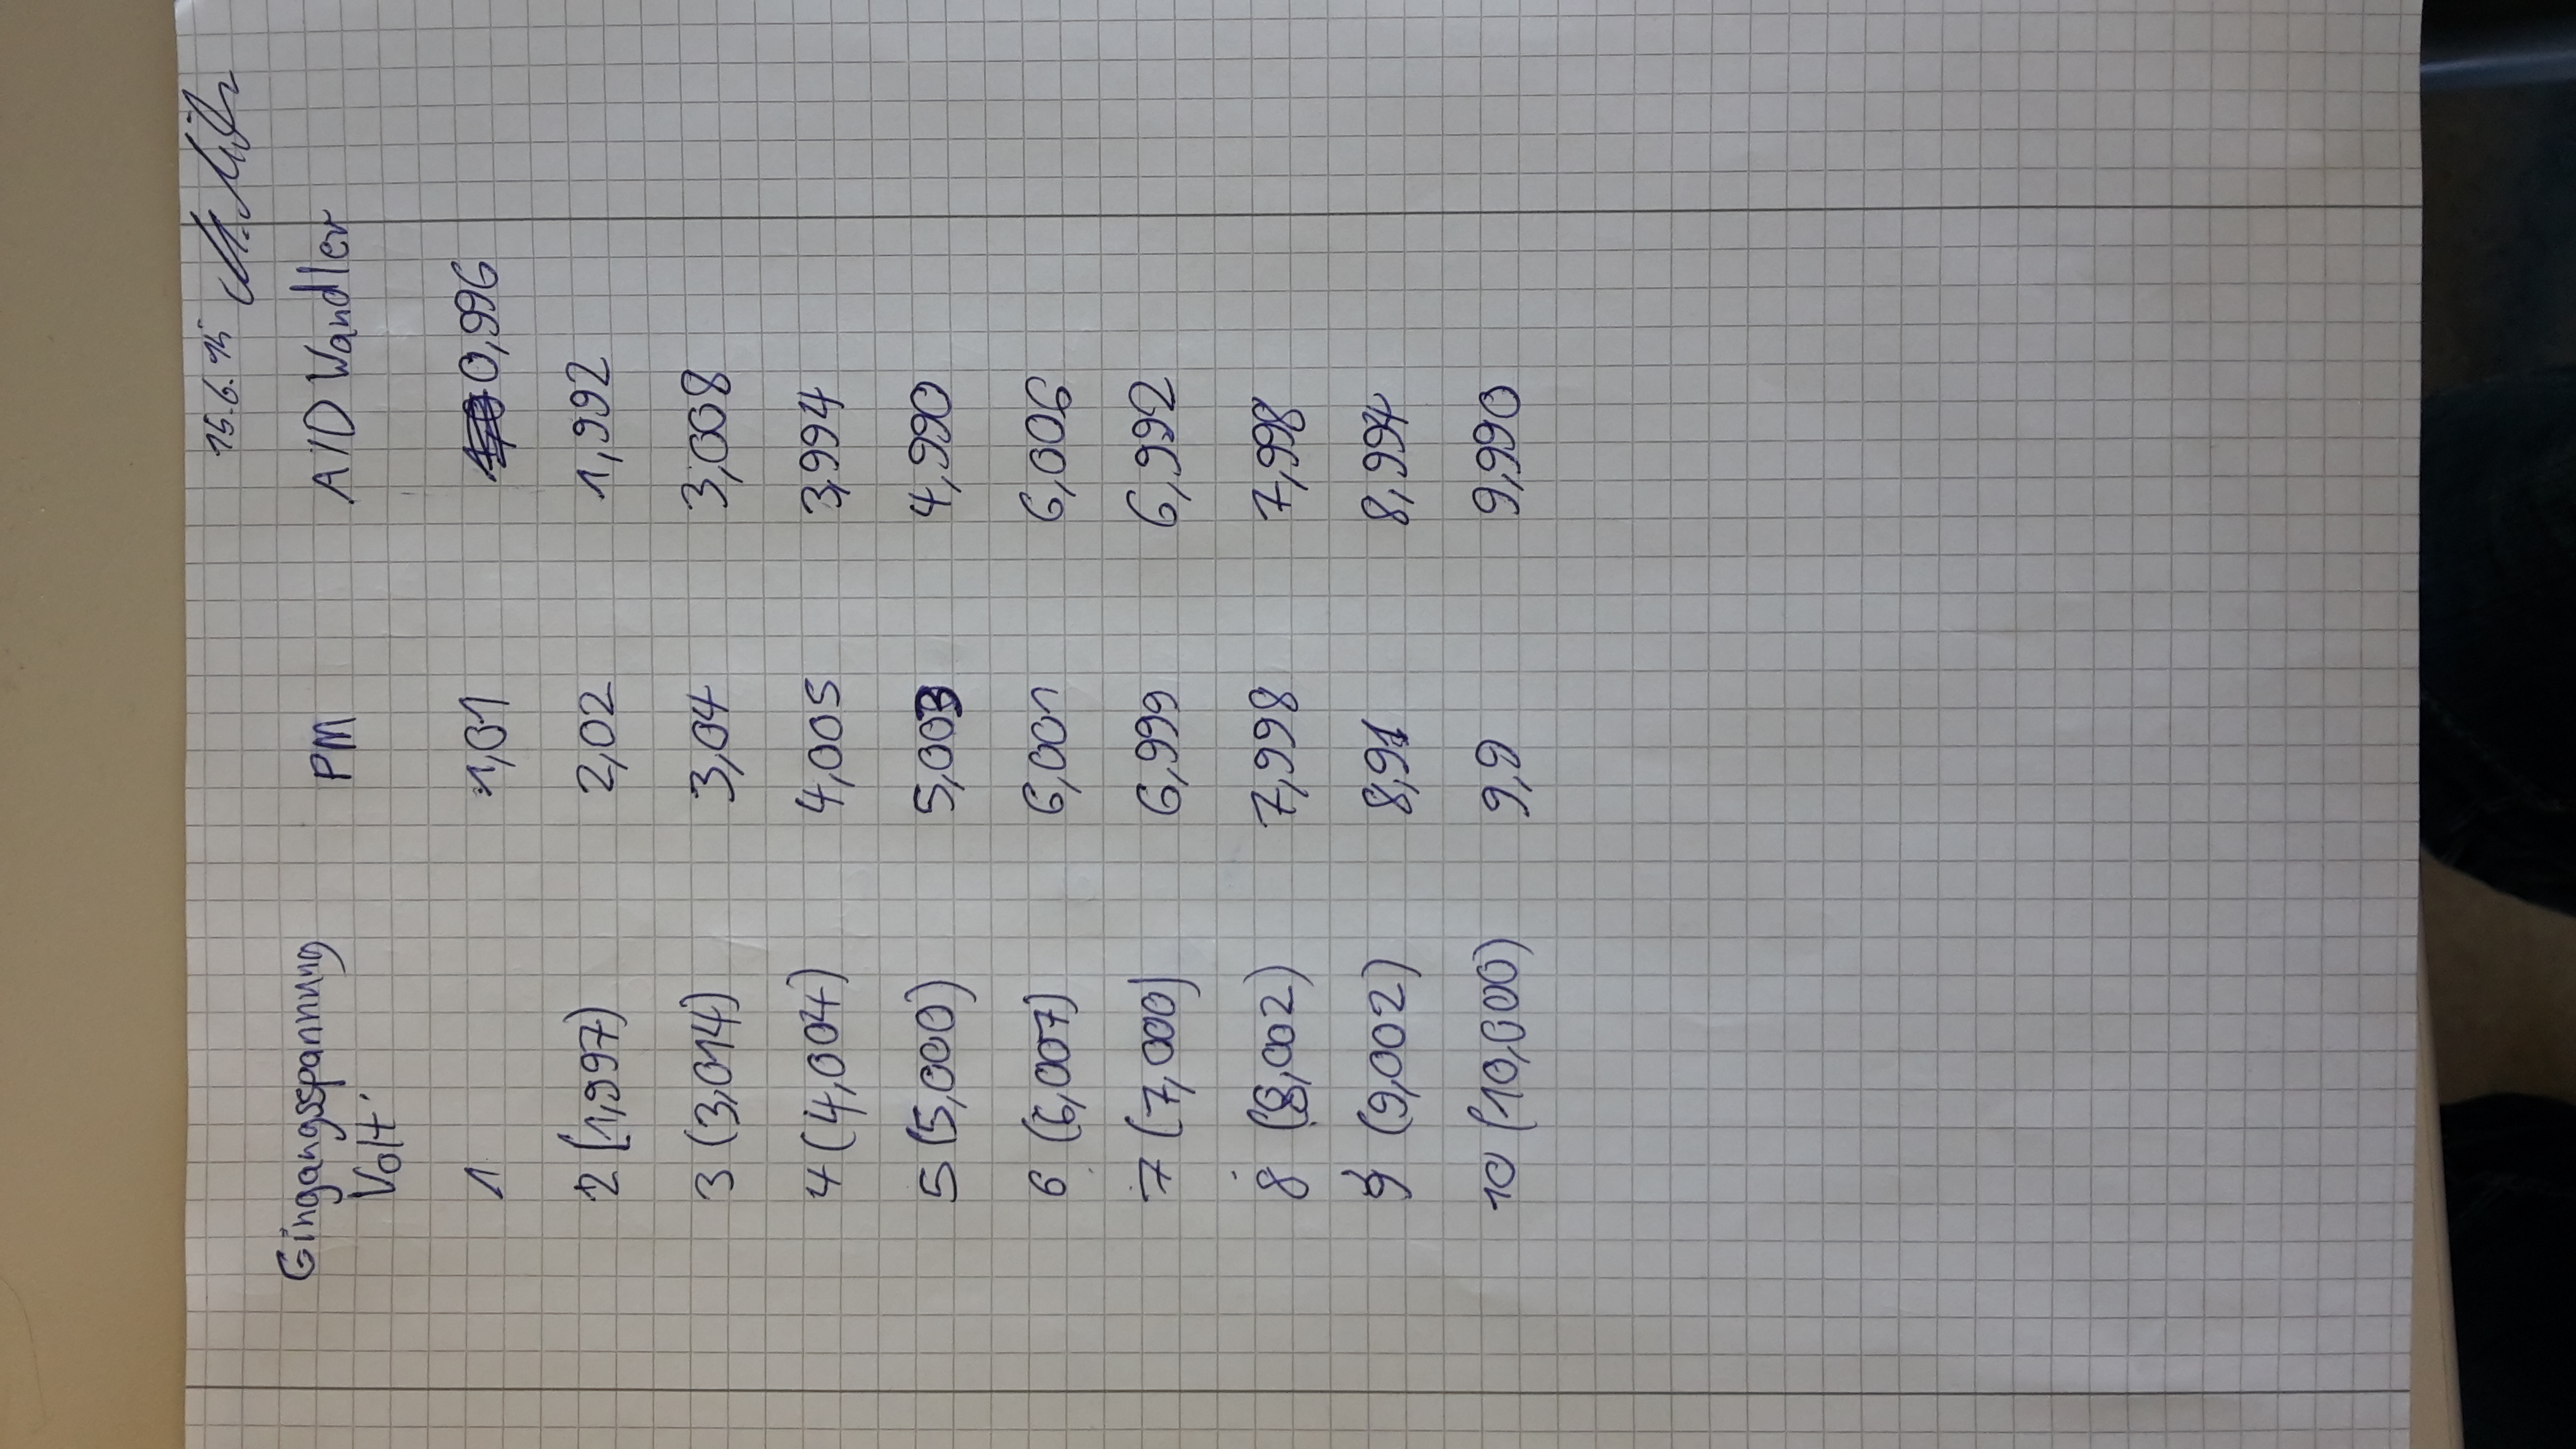
\includegraphics[width=1.5\textwidth, angle = -90]{media/Messprotokoll3.jpg}
	\label{Messergebnisse}
	\caption{Messergebnisse}
\end{figure}


%\begin{lstlisting}[style=VHDL, frame=single, caption=System Simulation, captionpos=b, label=lst:sys_sim]
%-- ADC Test Suite System Testbench
%--
%-- Author: Martin Miller
%-- Date:   16.08.2014
%-- 
%
%ENTITY system_tb IS
%   -- empty
%END system_tb;
%
%\end{lstlisting}

\clearpage

\end{document}